\documentclass[SoftwareDesign/SoftwareDesign_main.tex]{subfiles}

\begin{document}
\section{Design af Send Request ViewModel}
Når bruger/lejer har trykket på en bil inde fra SearchView bliver han dirigeret til SendRequest Viewet. Her har SendRequest viewmodel til formål at hente information om bilen, der er blevet trykket på i SearchViewet. Information om bilen bliver sendt med fra SearchViewet, da SendRequest viewmodel har abonneret på en Event Aggregator, som SearchViewModel udsender information til. Informationen vil ved hjælp af databinding blive vist på venstre side af SendRequestViewet. På højre side vil information til udlejer indtastes og herefter sendes til udlejer, hvos informationen er indtastet korrekt. På figur \ref{fig:sendrequestwirefram} ses en wireframe, som designet er gået ud fra. Det endelige resultat variere dog, da det på venstre side skulle vises lidt mere information end bare et billede.
\begin{figure}[H]
    \centering
    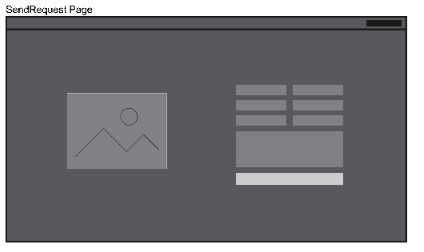
\includegraphics[width=\textwidth]{SoftwareDesign/MVVMDesigns/Graphics/SendRequestWireFrame.PNG}
    \caption{SendRequest WireFrame, som designet tager udgangspunkt i.}
    \label{fig:sendrequestwirefram}
\end{figure}

\subsection{UserControl med databinding}
For at få udskrevet information og tilbehør til bilen er der blevet lavet en UserControl, der ved hjælp af en ContentControl i SendRequestViewet fået sin egen CarProfilModel, hvor CarProfilModel er en property i SendRequestViewModel, som bliver initialiseret med værdier, når bil information hentes fra databasen. For at vise noget af informationen i CarProfileModel i til brugeren gøres brug af en valueconverter for at vise en boolean værdi i CarProfilModel. Her er true et check ikon og false er et advarsel symbol.
\subsection{Database Interaktion}
Når brugeren navigerer til SendRequest viewet fra SearchViewet skal SendRequest ViewModel udtrække information fra databasen om bilen og udlejeren af bilen. ViewModel bruger herefter denne information til at vise det på skærmen. Når lejer herefter har indtastet information om ønsket udlejningsdato fra og til, og eventuelt en besked, og trykket "Rent Car", så vil information gemmes i databasen, hvis der ikke er fejl i det indtastede information eller bilen allerede er udlejet i perioden. 
\subsection{Fejlhåndtering}
En vigtig ting i vores applikation er fejlhåndtering, så vi ikke gemmer forkert data i databasen eller information, der ikke giver mening. Dette bliver håndteret ved at applikationen textbox'ene og DatePicker kontrollerne bliver røde i kanten og fejlen nævnes i en tooltip. Det er heller ikke muligt trykke på knappen "Rent Car". Her vil brugeren informeres med rød tekst under knappen, hvis information er forkert indtastet. Der bliver også undersøgt om bilen allerede er udlejet i perioden, hvis dette er tilfældet bliver brugeren også informeret med rød skrift.
\end{document}